\documentclass[conference]{IEEEtran}
% QONTOS Research Paper Series — Shared LaTeX Preamble
% Use with: % QONTOS Research Paper Series — Shared LaTeX Preamble
% Use with: % QONTOS Research Paper Series — Shared LaTeX Preamble
% Use with: \input{qontos-preamble}

\usepackage{cite}
\usepackage{amsmath,amssymb,amsfonts}
\usepackage{graphicx}
\usepackage{textcomp}
\usepackage{xcolor}
\usepackage{hyperref}
\usepackage{booktabs}
\usepackage{multirow}
\usepackage{array}
\usepackage{tabularx}
\usepackage{float}
\usepackage{listings}
\usepackage{url}
\usepackage{enumitem}

% Listing style
\lstset{
  basicstyle=\ttfamily\footnotesize,
  breaklines=true,
  frame=single,
  backgroundcolor=\color{gray!10},
}

% Custom column type
\newcolumntype{L}[1]{>{\raggedright\arraybackslash}p{#1}}

% QONTOS colors
\definecolor{qontosnavy}{HTML}{0A1628}
\definecolor{qontosblue}{HTML}{1E88E5}
\definecolor{qontosteal}{HTML}{00BCD4}

% Hyperref setup
\hypersetup{
  colorlinks=true,
  linkcolor=qontosblue,
  citecolor=qontosblue,
  urlcolor=qontosteal,
}

% Author block
\newcommand{\qontosauthor}{%
\IEEEauthorblockN{QONTOS Research Wing}
\IEEEauthorblockA{
Zhyra Quantum Research Institute (ZQRI)\\
Advanced Quantum Systems Division\\
Abu Dhabi, UAE\\
\texttt{research@zhyra.xyz}}
}


\usepackage{cite}
\usepackage{amsmath,amssymb,amsfonts}
\usepackage{graphicx}
\usepackage{textcomp}
\usepackage{xcolor}
\usepackage{hyperref}
\usepackage{booktabs}
\usepackage{multirow}
\usepackage{array}
\usepackage{tabularx}
\usepackage{float}
\usepackage{listings}
\usepackage{url}
\usepackage{enumitem}

% Listing style
\lstset{
  basicstyle=\ttfamily\footnotesize,
  breaklines=true,
  frame=single,
  backgroundcolor=\color{gray!10},
}

% Custom column type
\newcolumntype{L}[1]{>{\raggedright\arraybackslash}p{#1}}

% QONTOS colors
\definecolor{qontosnavy}{HTML}{0A1628}
\definecolor{qontosblue}{HTML}{1E88E5}
\definecolor{qontosteal}{HTML}{00BCD4}

% Hyperref setup
\hypersetup{
  colorlinks=true,
  linkcolor=qontosblue,
  citecolor=qontosblue,
  urlcolor=qontosteal,
}

% Author block
\newcommand{\qontosauthor}{%
\IEEEauthorblockN{QONTOS Research Wing}
\IEEEauthorblockA{
Zhyra Quantum Research Institute (ZQRI)\\
Advanced Quantum Systems Division\\
Abu Dhabi, UAE\\
\texttt{research@zhyra.xyz}}
}


\usepackage{cite}
\usepackage{amsmath,amssymb,amsfonts}
\usepackage{graphicx}
\usepackage{textcomp}
\usepackage{xcolor}
\usepackage{hyperref}
\usepackage{booktabs}
\usepackage{multirow}
\usepackage{array}
\usepackage{tabularx}
\usepackage{float}
\usepackage{listings}
\usepackage{url}
\usepackage{enumitem}

% Listing style
\lstset{
  basicstyle=\ttfamily\footnotesize,
  breaklines=true,
  frame=single,
  backgroundcolor=\color{gray!10},
}

% Custom column type
\newcolumntype{L}[1]{>{\raggedright\arraybackslash}p{#1}}

% QONTOS colors
\definecolor{qontosnavy}{HTML}{0A1628}
\definecolor{qontosblue}{HTML}{1E88E5}
\definecolor{qontosteal}{HTML}{00BCD4}

% Hyperref setup
\hypersetup{
  colorlinks=true,
  linkcolor=qontosblue,
  citecolor=qontosblue,
  urlcolor=qontosteal,
}

% Author block
\newcommand{\qontosauthor}{%
\IEEEauthorblockN{QONTOS Research Wing}
\IEEEauthorblockA{
Zhyra Quantum Research Institute (ZQRI)\\
Advanced Quantum Systems Division\\
Abu Dhabi, UAE\\
\texttt{research@zhyra.xyz}}
}


\begin{document}

\title{QONTOS Scaled Quantum Architecture: A Scenario-Based Analysis of a Modular Path to 1 Million Physical Qubits}
\author{\qontosauthor}
\maketitle

\begin{abstract}
We analyze a stretch-case target for the QONTOS hybrid superconducting-photonic modular quantum computing architecture, examining the technical conditions under which a four-tier hierarchy of superconducting chiplets, cryogenic modules, photonically-interconnected systems, and data centers could scale to \textbf{1,000,000 physical qubits} supporting up to \textbf{10,000 logical qubits}. The architecture employs a canonical composition: chiplet (2,000 physical qubits) to module (5 chiplets, 10,000 qubits) to system (10 photonically-interconnected modules, 100,000 qubits) to data center (10 systems, 1,000,000 qubits). Achieving the full stretch target requires simultaneous advances in qubit coherence to the millisecond regime~\cite{bland2025}, two-qubit gate fidelities approaching 99.99\% or better~\cite{acharya2024}, error-correction overhead reduction toward an effective 100:1 physical-to-logical ratio~\cite{bravyi2024,googleqai2023}, high-rate photonic interconnects between cryogenic modules~\cite{monroe2014}, and scalable classical decoding within microsecond-class latency budgets~\cite{fowler2012}. We present base, aggressive, and stretch scenarios with explicit validation gates, no-go conditions, dependencies, and failure modes. All architectural figures in this paper represent planning targets; none have been experimentally demonstrated at scale.

\textbf{Claim status:} Architecture target and stretch scenario, informed by published literature and QONTOS internal planning. No experimental demonstrations of the full architecture are claimed.
\end{abstract}

\begin{IEEEkeywords}
quantum computing, modular architecture, fault-tolerant quantum computing, surface codes, quantum LDPC codes, distributed quantum systems, scenario planning, superconducting qubits, photonic interconnects, hybrid superconducting-photonic architecture
\end{IEEEkeywords}

%% ----------------------------------------------------------------
\section{Introduction}

\subsection{Motivation: Why Modular Scale Matters}

The path to large-scale, fault-tolerant quantum computation is constrained by at least five concurrent engineering challenges:

\begin{enumerate}
\item \textbf{Chip yield and frequency crowding.} Superconducting qubit processors face declining yield as qubit count grows on a monolithic die, driven by fabrication defects and frequency collision probability~\cite{koch2007}.

\item \textbf{Thermal load and wiring density.} Each qubit requires multiple microwave control lines and readout channels routed through a dilution refrigerator. At the scale of thousands of qubits, the thermal budget at the mixing chamber stage (typically 10--20~mK) becomes a binding constraint~\cite{ibm2024}.

\item \textbf{Error-correction overhead.} Current surface code implementations require on the order of 1,000 physical qubits per logical qubit at experimentally demonstrated error rates~\cite{fowler2012}. Reducing this overhead to practical levels requires simultaneous improvements in physical error rates and code efficiency.

\item \textbf{Inter-module communication fidelity.} Any modular architecture must solve the problem of high-fidelity entanglement distribution between physically separated cryogenic modules. Microwave-to-optical transduction efficiencies remain below 10\% in most reported experiments [Derived from literature].

\item \textbf{Classical decoder and control latency.} Real-time syndrome decoding must keep pace with the quantum error correction cycle. For superconducting qubits with microsecond-scale gate times, decoder latency budgets are on the order of 1~$\mu$s or less~\cite{krinner2022}.
\end{enumerate}

Monolithic architectures face increasing stress on all five fronts as qubit count rises. QONTOS therefore treats modularity as a first-class design principle rather than a late-stage packaging decision. The modular approach draws on the conceptual framework of Monroe et al.~\cite{monroe2014}, who proposed large-scale modular architectures for trapped-ion systems, adapted here to a hybrid superconducting-photonic architecture where superconducting qubit modules are interconnected via photonic links.

\subsection{Architectural Thesis}

QONTOS proposes that a hybrid superconducting-photonic modular architecture---superconducting chiplets integrated into cryogenic modules, modules interconnected via photonic links into systems, and systems aggregated into data-center-scale deployments---can relax the individual scaling bottlenecks described above, provided that qubit quality, error correction, photonic interconnect performance, and cryogenic infrastructure all improve on coordinated timelines.

This thesis is not a prediction. It is a structured engineering target against which progress can be measured and scenarios can be evaluated.

\subsection{Scope and Claim Status}

This paper uses the following claim labels throughout. Every quantitative assertion in this document carries one of these labels.

\begin{table}[htbp]
\centering
\caption{Claim Label Definitions.}
\label{tab:claim_labels}
\begin{tabular}{lp{3cm}p{2.5cm}}
\toprule
\textbf{Label} & \textbf{Definition} & \textbf{Example} \\
\midrule
\textbf{Demonstrated} & Measured in QONTOS systems or directly supported by published experimental results with citations & $T_1 > 300$~$\mu$s in tantalum transmons~\cite{bland2025} \\
\textbf{Simulated} & Supported by QONTOS digital-twin or simulator modeling with stated assumptions & Module-level crosstalk projections \\
\textbf{Derived from literature} & Based on published external results or conservative extrapolation thereof & Surface code thresholds~\cite{fowler2012} \\
\textbf{QONTOS target} & Internal engineering objective not yet demonstrated & 300:1 effective overhead \\
\textbf{Stretch target} & Requires multiple major assumptions landing together; aspirational & 100:1 overhead, 1M qubits \\
\bottomrule
\end{tabular}
\end{table}

\textbf{Overarching claim status for this paper:} The four-tier architecture and its million-qubit endpoint are \textbf{stretch targets}. The base and aggressive scenarios represent nearer-term planning configurations. No experimental demonstration of the full architecture is claimed.

\textbf{Architecture Claim Summary:}

\begin{table}[htbp]
\centering
\caption{Architecture Claim Summary.}
\label{tab:arch_claims}
\begin{tabular}{lp{3cm}}
\toprule
\textbf{Claim} & \textbf{Status} \\
\midrule
QONTOS uses a four-tier modular hierarchy & QONTOS target \\
2,000 physical qubits per chiplet & Stretch target \\
10,000 physical qubits per module (5 chiplets) & Stretch target \\
100,000 physical qubits per system (10 modules) & Stretch target \\
1,000,000 physical qubits per data center (10 systems) & Stretch target \\
10,000 logical qubits at 100:1 overhead & Stretch target \\
100:1 effective physical-to-logical overhead & Stretch target \\
\bottomrule
\end{tabular}
\end{table}

\subsection{Relationship to Other QONTOS Papers}

This architecture paper serves as the canonical reference for system composition numbers. Other papers in the QONTOS research series address specific subsystems:

\begin{itemize}
\item Paper~02: Tantalum-on-silicon qubit platform and coherence targets
\item Paper~03: Error correction and the path to 100:1 overhead
\item Paper~04: Photonic interconnects and modular entanglement distribution
\item Paper~05: AI-assisted decoding and classical control
\item Paper~06: Software stack and orchestration layer
\item Paper~07: Cryogenic infrastructure at scale
\item Paper~08: Quantum algorithms and applications
\item Paper~09: Benchmarking methodology
\item Paper~10: Integrated roadmap to 2030
\end{itemize}

All subsystem papers inherit the architecture constants defined in Section~\ref{sec:canonical}.

%% ----------------------------------------------------------------
\section{Background and Literature Context}

\subsection{Superconducting Qubit State of the Art}

The transmon qubit, introduced by Koch et al.~\cite{koch2007}, remains the dominant superconducting qubit modality for scalable quantum computing. Its charge-insensitive design, derived from the Cooper pair box, provides a favorable balance between coherence, controllability, and fabrication reproducibility.

Recent advances in materials science have pushed coherence times into the millisecond regime. Bland et al.~\cite{bland2025} reported $T_1$ relaxation times up to 1.68~ms in tantalum-on-silicon transmon qubits, representing an order-of-magnitude improvement over the typical 50--200~$\mu$s $T_1$ times achieved with conventional niobium-based fabrication on silicon or sapphire substrates. This result establishes that millisecond-class coherence is physically achievable in individual devices, though maintaining such performance at scale (hundreds or thousands of qubits on a single die with dense wiring) remains an open challenge.

Two-qubit gate fidelities have also improved substantially. Google Quantum AI (Acharya et al.~\cite{acharya2024}) demonstrated surface code operation with physical error rates below the threshold required for exponential suppression of logical errors with increasing code distance, representing a landmark result for the field. Their work showed that increasing the code distance from 3 to 5 to 7 yields the expected exponential improvement in logical error rate, confirming below-threshold operation. IBM's quantum-centric supercomputing roadmap~\cite{ibm2024, ibm2024b} projects systems with modular architectures combining classical and quantum processing, targeting utility-scale workloads.

These results establish that the individual qubit-level building blocks for large-scale fault-tolerant systems are approaching the required quality, though significant gaps remain in scaling these results to thousands of qubits on a single die and in maintaining performance under the wiring and thermal constraints of large integrated systems.

\subsection{Error Correction: Surface Codes and Beyond}

The surface code, analyzed comprehensively by Fowler et al.~\cite{fowler2012}, is the most mature approach to fault-tolerant quantum computation with superconducting qubits. It offers a relatively high error threshold (approximately 1\%) and requires only nearest-neighbor connectivity on a 2D lattice, making it naturally compatible with planar superconducting qubit layouts.

However, surface codes carry substantial overhead. At physical error rates of approximately $10^{-3}$, achieving a logical error rate suitable for useful computation (e.g., $10^{-10}$ for applications such as quantum chemistry or Shor's algorithm) requires code distances on the order of $d = 17$--25. This corresponds to roughly 600--1,250 physical qubits per logical qubit for the data block alone, plus ancilla overhead for syndrome extraction. When accounting for magic state distillation (required for universal computation), lattice surgery routing, and other operational overheads, effective ratios of 1,000:1 or higher are typical in current analyses~\cite{fowler2012, chamberland2022}.

Recent theoretical advances in quantum low-density parity-check (qLDPC) codes offer the possibility of asymptotically better overhead scaling. Panteleev and Kalachev~\cite{panteleev2022} demonstrated the existence of asymptotically good quantum LDPC codes---codes with constant rate and linear distance---resolving a long-standing open question in quantum coding theory. Bravyi et al.~\cite{bravyi2024} demonstrated high-threshold, low-overhead quantum memory using a specific qLDPC construction, achieving a storage threshold of approximately 0.7\% with overhead substantially below surface code levels. However, translating these theoretical results to a full fault-tolerant computation (including magic state injection and logical gate operations) on physical hardware remains an open research problem.

Experimentally, Krinner et al.~\cite{krinner2022} demonstrated repeated quantum error correction in a distance-three surface code on a superconducting processor, establishing experimental precedent for real-time QEC cycles. Acharya et al.~\cite{acharya2024} subsequently demonstrated that increasing the code distance from 3 to 5 to 7 reduces logical error rates exponentially, confirming below-threshold operation in a superconducting platform. These results validate the surface code approach but also underscore the scale of overhead involved at current error rates.

The QONTOS architecture assumes that the effective physical-to-logical overhead will decrease over the program lifetime as physical error rates improve and as more efficient codes (potentially qLDPC) become practically implementable on hardware.

\subsection{Modular and Distributed Quantum Architectures}

Monroe et al.~\cite{monroe2014} articulated the foundational case for modular quantum computer architectures, arguing that photonic interconnects between small quantum processor nodes could circumvent the scaling limitations of monolithic designs. While their analysis focused on trapped-ion systems, the modular principle translates to superconducting platforms with appropriate modifications to the interconnect technology.

For superconducting qubits, modularity introduces the challenge of microwave-to-optical transduction. Efficient, low-noise conversion between microwave photons (typically 5--8~GHz, the natural operating frequency of transmon qubits) and optical photons (suitable for low-loss fiber transmission and room-temperature routing) remains an active area of research. Current state-of-the-art transduction efficiencies are typically below 10\% for end-to-end processes, though individual conversion steps have demonstrated higher performance in isolated experiments [Derived from literature].

Chamberland et al.~\cite{chamberland2022} analyzed the full system-level requirements for building a fault-tolerant quantum computer using concatenated codes, including the interplay between physical error rates, code distances, magic state distillation overhead, and decoder throughput. Their analysis provides a useful framework for understanding the gap between current capabilities and fault-tolerant operation at the scale required for useful applications.

\subsection{Classical Control and Decoding}

Real-time decoding of error correction syndromes is a computationally demanding task that must be completed within the error correction cycle time. For superconducting qubits with gate times on the order of 20--100~ns and measurement times on the order of 0.5--1~$\mu$s, the decoder must process syndrome data and determine corrections within a budget of roughly 1~$\mu$s. Exceeding this budget causes a syndrome backlog that degrades the effective logical error rate [Derived from literature].

Approaches to high-speed decoding include lookup-table decoders (fast but memory-limited at large code distances), union-find decoders (efficient average-case complexity), and machine-learning-assisted decoders (potentially faster inference at the cost of training complexity). The QONTOS approach to AI-assisted decoding is detailed in Paper~05 of this series.

%% ----------------------------------------------------------------
\section{Canonical Architecture Constants}
\label{sec:canonical}

This section is the \textbf{canonical source} for architecture composition numbers across the entire QONTOS research paper set. All other papers inherit these definitions.

\subsection{Four-Tier Hierarchy Definition}

\begin{figure}[htbp]
\centering
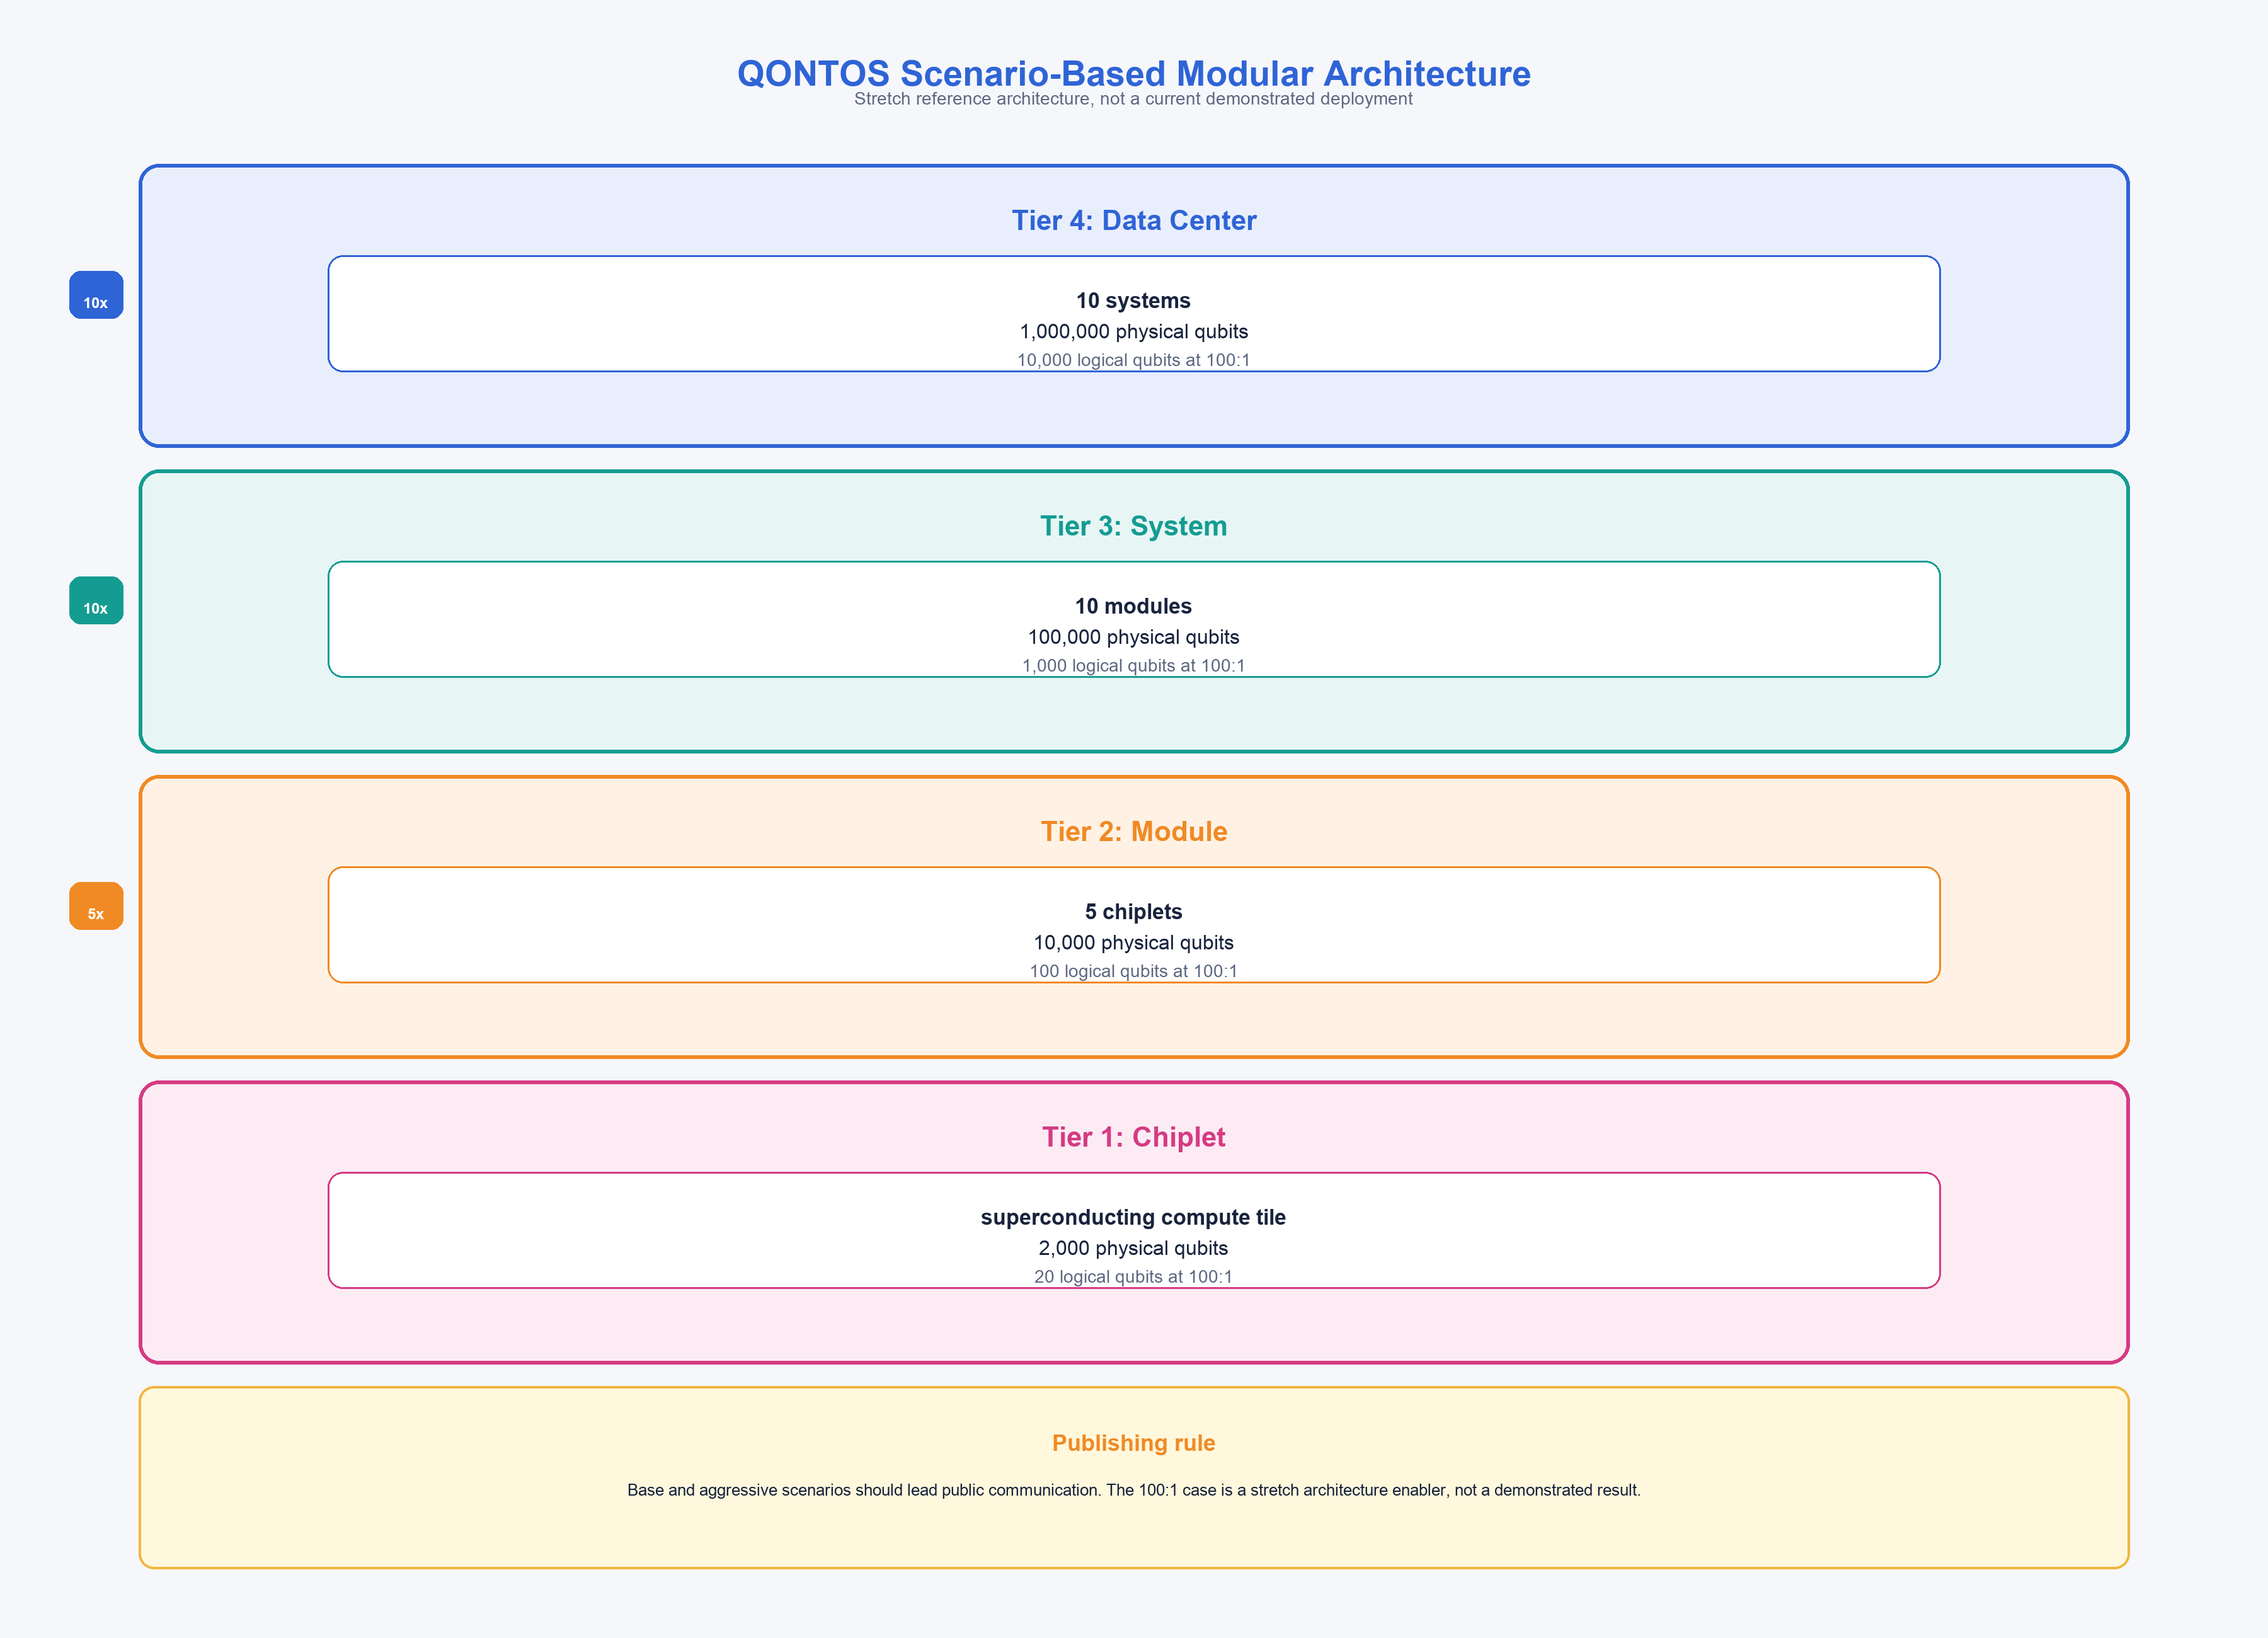
\includegraphics[width=\columnwidth]{../../figures/01_complete_architecture.png}
\caption{Four-Tier Modular Architecture.}
\label{fig:four_tier}
\end{figure}

The QONTOS stretch architecture defines a four-tier modular hierarchy:

\begin{table}[htbp]
\centering
\caption{Four-Tier Modular Hierarchy (Stretch).}
\label{tab:hierarchy}
\begin{tabular}{llrrp{1.8cm}}
\toprule
\textbf{Layer} & \textbf{Composition} & \textbf{Phys.\ Qubits} & \textbf{Log.\ (100:1)} & \textbf{Claim Status} \\
\midrule
Chiplet & 1 SC die & 2,000 & 20 & Stretch target \\
Module & 5 chiplets & 10,000 & 100 & Stretch target \\
System & 10 modules & 100,000 & 1,000 & Stretch target \\
Data Ctr. & 10 systems & 1,000,000 & 10,000 & Stretch target \\
\bottomrule
\end{tabular}
\end{table}

\textbf{Arithmetic verification:}
\begin{itemize}
\item $2{,}000 \times 5 = 10{,}000$ (chiplet to module)
\item $10{,}000 \times 10 = 100{,}000$ (module to system)
\item $100{,}000 \times 10 = 1{,}000{,}000$ (system to data center)
\item The data center comprises \textbf{10 systems}, not 100.
\item At 100:1 overhead: $1{,}000{,}000 / 100 = 10{,}000$ logical qubits.
\end{itemize}

\subsection{Tier 1: QPU Chiplet}

The chiplet is the fundamental fabricated superconducting qubit die.

\begin{table}[htbp]
\centering
\caption{Tier~1 Chiplet Parameters (Stretch).}
\label{tab:chiplet}
\begin{tabular}{lllp{2.2cm}}
\toprule
\textbf{Parameter} & \textbf{Value} & \textbf{Claim} & \textbf{Notes} \\
\midrule
Physical qubits & 2,000 & Stretch & High-yield fab at scale \\
Logical qubits & 20 & Stretch & Conditional on QEC \\
Die size & 15--20~mm/side & Target & Not validated \\
Qubit modality & Transmon (Ta-on-Si) & Target & Koch et al.~\cite{koch2007}; Bland et al.~\cite{bland2025} \\
Topology & Heavy-hex or equiv. & Target & Surface code / qLDPC \\
$T_1$ coherence & $> 1$~ms & Stretch & Up to 1.68~ms demo.~\cite{bland2025} \\
$T_2$ coherence & $> 500$~$\mu$s & Stretch & Echo techniques \\
1Q gate fidelity & $> 99.99\%$ & Target & Demo.\ on isolated devices \\
2Q gate fidelity & $> 99.9\%$ & Target & Demo.\ at moderate scale~\cite{acharya2024} \\
Readout fidelity & $> 99.5\%$ & Target & Multiplexed config.\ \\
Ctrl lines/qubit & ${\sim}2.5$ & Lit.\ & Wiring density \\
\bottomrule
\end{tabular}
\end{table}

\textbf{Key risks at Tier~1:} Frequency crowding at 2,000-qubit density; yield degradation on larger die; coherence reduction from increased wiring and crosstalk.

\subsection{Tier 2: Quantum Module}

The module is the cryogenic integration unit housing multiple chiplets within a single dilution refrigerator or cryogenic stage.

\begin{table}[htbp]
\centering
\caption{Tier~2 Module Parameters (Stretch).}
\label{tab:module}
\begin{tabular}{llp{3cm}}
\toprule
\textbf{Parameter} & \textbf{Value} & \textbf{Notes} \\
\midrule
Chiplets/module & 5 & Architecture constant \\
Physical qubits & 10,000 & $5 \times 2{,}000$ \\
Logical qubits & 100 & Conditional on QEC \\
Inter-chiplet coupling & MW or short-range galvanic & $> 99.5\%$ fidelity \\
Cryo.\ environment & Single DR, 10--20~mK & Cooling for 5 chiplets \\
Classical control & Dedicated RT + cryo electronics & Multiplexed readout \\
\bottomrule
\end{tabular}
\end{table}

\textbf{Key risks at Tier~2:} Inter-chiplet coupling fidelity; thermal load from 5 chiplets exceeding dilution refrigerator capacity; signal integrity degradation in dense multi-chiplet packaging.

\subsection{Tier 3: Quantum System}

The system is the first tier employing photonic interconnects to link physically separated cryogenic modules.

\begin{table}[htbp]
\centering
\caption{Tier~3 System Parameters (Stretch).}
\label{tab:system}
\begin{tabular}{llp{2.5cm}}
\toprule
\textbf{Parameter} & \textbf{Value} & \textbf{Notes} \\
\midrule
Modules/system & 10 & Architecture constant \\
Physical qubits & 100,000 & $10 \times 10{,}000$ \\
Logical qubits & 1,000 & Conditional on QEC + interconnect \\
Inter-module link & Optical/photonic & MW-to-optical transduction \\
Transd.\ efficiency & $> 20\%$ (stretch) & Lit.\ reports $< 10\%$ \\
Entangl.\ gen.\ rate & $> 10$~kHz/link & For distributed QEC \\
Classical backbone & High-BW, low-latency & Syndrome + control \\
\bottomrule
\end{tabular}
\end{table}

\textbf{Key risks at Tier~3:} Transduction efficiency insufficient for distributed QEC; entanglement rate too low for practical cross-module operations; classical control latency across modules exceeds decoder budget.

\subsection{Tier 4: Quantum Data Center}

The data center is the facility-scale stretch endpoint.

\begin{table}[htbp]
\centering
\caption{Tier~4 Data Center Parameters (Stretch).}
\label{tab:datacenter}
\begin{tabular}{llp{2.5cm}}
\toprule
\textbf{Parameter} & \textbf{Value} & \textbf{Notes} \\
\midrule
Systems/data center & 10 & Yields 1M qubits \\
Physical qubits & 1,000,000 & $10 \times 100{,}000$ \\
Logical qubits & 10,000 & Full stretch scenario \\
Power consumption & ${\sim}1$~MW & Planning estimate \\
Facility footprint & ${\sim}100$--$200~\text{m}^2$ & Incl.\ cryo + classical \\
Cooling & Multiple large DRs & Novel cryo engineering \\
Classical HPC & Integrated supercomputer & Hybrid QC workloads \\
\bottomrule
\end{tabular}
\end{table}

\textbf{Key risks at Tier~4:} Facility power and cooling costs; manufacturing and integration complexity at scale; operational reliability across 10 concurrent systems.

\subsection{Architecture Arithmetic Verification}

\begin{table}[htbp]
\centering
\caption{Architecture Arithmetic Across Scenarios.}
\label{tab:arithmetic}
\begin{tabular}{lrrr}
\toprule
\textbf{Calculation} & \textbf{Base} & \textbf{Aggr.} & \textbf{Stretch} \\
\midrule
Qubits/chiplet & 500 & 1,000 & 2,000 \\
Chiplets/module & 5 & 5 & 5 \\
Qubits/module & 2,500 & 5,000 & 10,000 \\
Modules/system & 4 & 10 & 10 \\
Qubits/system & 10,000 & 50,000 & 100,000 \\
Systems/data ctr. & 2 & 10 & 10 \\
\textbf{Qubits/data ctr.} & \textbf{20,000} & \textbf{500,000} & \textbf{1,000,000} \\
Overhead ratio & 1,000:1 & 300:1 & 100:1 \\
\textbf{Logical qubits} & \textbf{20} & \textbf{${\sim}$1,667} & \textbf{10,000} \\
\bottomrule
\end{tabular}
\end{table}

%% ----------------------------------------------------------------
\section{Error-Correction Envelope}

\subsection{Overhead Regimes and Their Implications}

The effective physical-to-logical qubit ratio is the single most consequential parameter for the architecture. It determines how many logical qubits---the units of useful computation---can be extracted from a given number of physical qubits.

\begin{table}[htbp]
\centering
\caption{Overhead Regimes.}
\label{tab:overhead}
\begin{tabular}{rllp{2cm}}
\toprule
\textbf{Regime} & \textbf{Phys./Log.} & \textbf{Claim} & \textbf{Context} \\
\midrule
1,000:1 & 1,000 & Lit.\ & Conservative baseline~\cite{fowler2012, chamberland2022} \\
300:1 & 300 & Target & Aggr.\ target, ${\sim}10^{-4}$ errors \\
100:1 & 100 & Stretch & Low errors + efficient codes \\
\bottomrule
\end{tabular}
\end{table}

\textbf{System-level implications for 1,000,000 physical qubits:}

\begin{table}[htbp]
\centering
\caption{Logical Qubit Yield from 1M Physical Qubits.}
\label{tab:logical_yield}
\begin{tabular}{rrp{3.5cm}}
\toprule
\textbf{Overhead} & \textbf{Logical Qubits} & \textbf{Application Class} \\
\midrule
1,000:1 & 1,000 & Early FT demos; small chemistry \\
300:1 & ${\sim}$3,333 & Intermediate chemistry; optimization \\
100:1 & 10,000 & Crypto-relevant; large-scale simulation \\
\bottomrule
\end{tabular}
\end{table}

\subsection{Surface Codes vs.\ Quantum LDPC Codes}

The path from 1,000:1 to 100:1 overhead likely requires a transition from standard surface codes to more efficient code families.

\begin{table}[htbp]
\centering
\caption{Code Family Overhead Comparison.}
\label{tab:code_families}
\begin{tabular}{lllp{1.5cm}}
\toprule
\textbf{Code Family} & \textbf{${\sim}10^{-3}$ err.} & \textbf{${\sim}10^{-4}$ err.} & \textbf{Status} \\
\midrule
Surface (standard) & 1,000--1,500:1 & 300--500:1 & Literature \\
Surface (optimized) & 800--1,000:1 & 200--400:1 & Literature \\
qLDPC (theoretical) & 200--500:1 & 50--150:1 & Literature \\
qLDPC (practical) & 300--500:1 & 100--200:1 & Stretch \\
\bottomrule
\end{tabular}
\end{table}

\textbf{Important caveat:} The qLDPC overhead figures are based on theoretical constructions and limited numerical studies. Practical implementation of qLDPC codes on superconducting hardware introduces non-local connectivity requirements that may conflict with planar chip topologies. The figures above should be treated as indicative, not predictive.

\subsection{Base / Aggressive / Stretch Scenarios}

\begin{table}[htbp]
\centering
\caption{Error-Correction Scenario Parameters.}
\label{tab:qec_scenarios}
\begin{tabular}{lrrr}
\toprule
\textbf{Parameter} & \textbf{Base} & \textbf{Aggr.} & \textbf{Stretch} \\
\midrule
Phys.\ error rate (2Q) & $10^{-3}$ & $5 \times 10^{-4}$ & $10^{-4}$ \\
Code family & Surface & Opt.\ surface & Surface + qLDPC \\
Effective overhead & 1,000:1 & 300:1 & 100:1 \\
Phys.\ qubits (DC) & 20,000 & 500,000 & 1,000,000 \\
Logical qubits & ${\sim}$20 & ${\sim}$1,667 & 10,000 \\
Target $p_L$ & $10^{-6}$ & $10^{-8}$ & $10^{-10}$ \\
Decoder latency & 10~$\mu$s & 1~$\mu$s & $< 1$~$\mu$s \\
\bottomrule
\end{tabular}
\end{table}

\subsection{Coupled Assumptions}

The 100:1 overhead target is not an independent parameter. It is coupled to a set of subsystem requirements that must all be met simultaneously:

\begin{table}[htbp]
\centering
\caption{Coupled Requirements for 100:1 Overhead.}
\label{tab:coupled}
\begin{tabular}{llp{2.5cm}}
\toprule
\textbf{Requirement} & \textbf{Threshold} & \textbf{Dependency} \\
\midrule
Phys.\ error rate (2Q) & $< 10^{-4}$ & Qubit quality, calibration \\
$T_1$ at scale & $> 1$~ms & Materials, fab, packaging \\
Code efficiency & $>$ surface code & Practical qLDPC \\
Decoder throughput & $< 1$~$\mu$s/round & FPGA/ASIC or ML \\
Measurement fidelity & $> 99.5\%$ & Mux.\ readout chain \\
\bottomrule
\end{tabular}
\end{table}

If any one of these requirements fails to improve sufficiently, the effective overhead rises, and the architecture delivers fewer logical qubits from the same physical qubit count. This is why the million-qubit architecture and the 100:1 assumption must always be presented as a \textbf{coupled stretch scenario}.

%% ----------------------------------------------------------------
\section{Scenario Framework}

\subsection{Three-Scenario Model}

\begin{table*}[htbp]
\centering
\caption{Three-Scenario Model (Complete).}
\label{tab:three_scenario}
\begin{tabular}{lrrrp{3cm}}
\toprule
\textbf{Metric} & \textbf{Base} & \textbf{Aggressive} & \textbf{Stretch} & \textbf{Claim Status} \\
\midrule
Phys.\ qubits/chiplet & 500 & 1,000 & 2,000 & Base: target; Stretch: stretch \\
Chiplets/module & 5 & 5 & 5 & Architecture constant \\
Phys.\ qubits/module & 2,500 & 5,000 & 10,000 & Derived \\
Modules/system & 4 & 10 & 10 & Base: target; Aggr.+: stretch \\
Phys.\ qubits/system & 10,000 & 50,000 & 100,000 & Derived \\
Systems/data center & 2 & 10 & 10 & Base: target; Aggr.+: stretch \\
Phys.\ qubits/data ctr. & 20,000 & 500,000 & 1,000,000 & Derived \\
Effective overhead & 1,000:1 & 300:1 & 100:1 & See Section~4 \\
Logical qubits & ${\sim}$20 & ${\sim}$1,667 & 10,000 & Derived \\
$T_1$ coherence (at scale) & 200~$\mu$s & 500~$\mu$s & $> 1$~ms & Lit.\ to stretch \\
2Q gate fidelity & 99.9\% & 99.95\% & 99.99\% & Lit.\ to stretch \\
Transd.\ efficiency & N/A & 5--10\% & $> 20\%$ & Lit.\ to stretch \\
Decoder latency & 10~$\mu$s & 1~$\mu$s & $< 1$~$\mu$s & Target to stretch \\
\bottomrule
\end{tabular}
\end{table*}

\subsection{Scenario-Based Performance Table}

\begin{table*}[htbp]
\centering
\caption{Scenario-Based Performance Estimates.}
\label{tab:performance}
\begin{tabular}{llllp{3cm}}
\toprule
\textbf{Metric} & \textbf{Base} & \textbf{Aggressive} & \textbf{Stretch} & \textbf{Notes} \\
\midrule
Quantum volume (est.) & $2^{10}$--$2^{15}$ & $2^{20}$--$2^{30}$ & $2^{40}$+ & Order-of-magnitude \\
Circuit depth (logical) & ${\sim}10^2$ & ${\sim}10^4$ & ${\sim}10^6$ & Before decoherence \\
Logical clock rate (ops/s) & ${\sim}10^3$ & ${\sim}10^4$ & ${\sim}10^5$ & QEC cycle time \\
Application class & Small variational & Intermed.\ chemistry & Crypto-relevant & Illustrative \\
Est.\ power (data ctr.) & ${\sim}100$~kW & ${\sim}500$~kW & ${\sim}1$~MW & Facility planning \\
Est.\ footprint & ${\sim}20~\text{m}^2$ & ${\sim}50~\text{m}^2$ & ${\sim}100$--$200~\text{m}^2$ & Facility planning \\
\bottomrule
\end{tabular}
\end{table*}

\subsection{Validation Gates}

Each gate represents a decision point at which the program trajectory is evaluated against experimental evidence.

\begin{table*}[htbp]
\centering
\caption{Validation Gates.}
\label{tab:gates}
\begin{tabular}{lp{4cm}p{3.5cm}p{4cm}}
\toprule
\textbf{Gate} & \textbf{Criterion} & \textbf{Why It Matters} & \textbf{Evaluation Method} \\
\midrule
G1: Device Metrics & $T_1 > 500$~$\mu$s and 2Q fidelity $> 99.9\%$ on QONTOS devices & Architecture cannot scale without qubit quality & Experimental measurement; statistical significance \\
G2: Logical Qubit & First logical qubit on multi-chiplet module with lifetime exceeding physical qubits & Modular integration must be validated end-to-end & Logical qubit lifetime measurement \\
G3: Inter-Module Entangl. & Bell state fidelity $> 90\%$ across photonic link & Architecture fails if modular links underperform & Bell state tomography \\
G4: Digital Twin & Simulator predictions match experiments within 20\% & Planning becomes guesswork without validated models & Systematic comparison \\
G5: Economic Viability & Cost per logical qubit consistent with application value & Million-qubit narrative fails if costs are prohibitive & Cost model validation \\
\bottomrule
\end{tabular}
\end{table*}

\subsection{No-Go Conditions}

The stretch scenario should be formally downgraded if any of the following conditions persist beyond the PIONEER phase (2027--2028):

\begin{enumerate}
\item \textbf{Overhead stagnation:} Effective overhead remains closer to 1,000:1 than to 300:1 despite best efforts on physical error rates and code optimization.
\item \textbf{Transduction failure:} Microwave-to-optical transduction efficiency remains in low-single-digit percentages, precluding practical inter-module entanglement at rates required for distributed error correction.
\item \textbf{Packaging limits:} Multi-chiplet integration at 10,000 qubits per module proves unmanageable due to yield, crosstalk, or thermal constraints.
\item \textbf{Cryogenic scaling failure:} Cooling power and control wiring cannot support the thermal load of multi-module systems at the 10-module scale.
\item \textbf{Decoder latency wall:} Classical decoding cannot keep pace with the QEC cycle time even with dedicated hardware acceleration (FPGA, ASIC, or ML approaches).
\end{enumerate}

%% ----------------------------------------------------------------
\section{Dependencies and Assumptions}

\subsection{Technology Dependencies}

\begin{table*}[htbp]
\centering
\caption{Technology Dependencies by Scenario.}
\label{tab:tech_deps}
\begin{tabular}{lllll}
\toprule
\textbf{Dependency} & \textbf{Base} & \textbf{Aggressive} & \textbf{Stretch} & \textbf{Status (2026)} \\
\midrule
Qubit coherence ($T_1$) & $> 200$~$\mu$s & $> 500$~$\mu$s & $> 1$~ms & $> 2$~ms isolated~\cite{bland2025} \\
2Q gate fidelity & $> 99.9\%$ & $> 99.95\%$ & $> 99.99\%$ & $> 99.9\%$ moderate scale~\cite{acharya2024} \\
Chiplet qubit count & 500 & 1,000 & 2,000 & ${\sim}1{,}000$+ (industry) \\
Multi-chiplet integr. & 2--3/module & 5/module & 5/module & Small scale demo~\cite{ibm2024b} \\
MW-to-optical transd. & Not req. & 5--10\% & $> 20\%$ & $< 10\%$ reported \\
qLDPC implementation & Not req. & Not req. & On hardware & Theory only~\cite{bravyi2024, panteleev2022} \\
Real-time decoding & 10~$\mu$s & 1~$\mu$s & $< 1$~$\mu$s & ${\sim}1$~$\mu$s small codes \\
Cryogenic scale & 1 large DR & 2--4 DRs & 10+ DRs & Single large DR operational \\
\bottomrule
\end{tabular}
\end{table*}

\subsection{Supply Chain and Fabrication Assumptions}

\begin{table}[htbp]
\centering
\caption{Supply Chain Assumptions.}
\label{tab:supply}
\begin{tabular}{lp{3cm}l}
\toprule
\textbf{Assumption} & \textbf{Description} & \textbf{Risk} \\
\midrule
Tantalum supply & Sufficient high-purity Ta & Low \\
Foundry access & 2,000-qubit chiplet fab & Medium \\
Packaging tech. & Multi-chiplet cryo packaging & High \\
Cryo hardware & DRs for 10k-qubit modules & Medium \\
Control electronics & Scalable RT + cryo control & Medium \\
Optical components & Low-loss transducers + fiber & High \\
\bottomrule
\end{tabular}
\end{table}

\subsection{Cryogenic and Facility Assumptions}

\begin{table}[htbp]
\centering
\caption{Cryogenic and Facility Assumptions.}
\label{tab:cryo}
\begin{tabular}{llp{2cm}}
\toprule
\textbf{Parameter} & \textbf{Assumption} & \textbf{Claim} \\
\midrule
MXC temperature & 10--20~mK & Demonstrated \\
Cooling power/module & $> 20$~$\mu$W & Target \\
Heat load/qubit & $< 1$~nW & Literature \\
RT electronics power & ${\sim}100$~W/1k qubits & Target \\
Total facility power & ${\sim}1$~MW for 1M qubits & Target (est.) \\
Facility availability & $> 95\%$ uptime & Target \\
He-3 supply & Sufficient for multiple DRs & Medium risk \\
\bottomrule
\end{tabular}
\end{table}

%% ----------------------------------------------------------------
\section{Risks and Failure Modes}

\subsection{Technical Risks}

\begin{table}[htbp]
\centering
\caption{Technical Risk Assessment.}
\label{tab:tech_risks}
\begin{tabular}{p{2cm}llp{2.3cm}}
\toprule
\textbf{Risk} & \textbf{Likelih.} & \textbf{Impact} & \textbf{Mitigation} \\
\midrule
Coherence doesn't scale & Medium & High & Materials R\&D; process control \\
2Q fidelity saturates & Medium & High & Multiple gate impls.; auto-calibration \\
qLDPC impractical on planar HW & Medium & Medium & Surface code fallback; 3D integration \\
Transd.\ efficiency insufficient & High & High & Multiple modalities; all-MW fallback \\
Decoder latency exceeds budget & Medium & Medium & FPGA/ASIC; AI-assisted decoding \\
Frequency crowding & Medium & High & Fab uniformity; tunable designs \\
\bottomrule
\end{tabular}
\end{table}

\subsection{Integration Risks}

\begin{table}[htbp]
\centering
\caption{Integration Risk Assessment.}
\label{tab:int_risks}
\begin{tabular}{p{2cm}llp{2.3cm}}
\toprule
\textbf{Risk} & \textbf{Likelih.} & \textbf{Impact} & \textbf{Mitigation} \\
\midrule
Packaging yield too low & Medium & High & Chiplet-level testing; KGD screening \\
Inter-chiplet crosstalk & Medium & High & EM shielding; digital-twin prediction \\
Classical ctrl.\ scaling & Medium & Medium & Hierarchical arch.; HPC partnerships \\
Cryo wiring density & Medium & High & Cryo multiplexing; cryo-CMOS \\
\bottomrule
\end{tabular}
\end{table}

\subsection{Programmatic Risks}

\begin{table}[htbp]
\centering
\caption{Programmatic Risk Assessment.}
\label{tab:prog_risks}
\begin{tabular}{p{2cm}llp{2.3cm}}
\toprule
\textbf{Risk} & \textbf{Likelih.} & \textbf{Impact} & \textbf{Mitigation} \\
\midrule
Timeline slippage & High & Medium & Scenario framework provides fallbacks \\
Competitor advantage & Medium & Medium & Differentiated SW + orchestration \\
Funding insufficient & Medium & High & Phased investment; demo value early \\
Key personnel deps. & Medium & Medium & Knowledge building; diversified partners \\
\bottomrule
\end{tabular}
\end{table}

\subsection{Mitigation Strategies}

The three-scenario framework is itself the primary risk mitigation strategy. By defining base, aggressive, and stretch targets with explicit validation gates, the program can adapt its trajectory without narrative collapse:

\begin{enumerate}
\item \textbf{If the stretch scenario fails}, the aggressive scenario still delivers a commercially relevant system with hundreds to thousands of logical qubits.
\item \textbf{If the aggressive scenario underperforms}, the base scenario still supports meaningful quantum computing demonstrations and a credible software platform.
\item \textbf{Validation gates (Section~5.3) provide early warning} of trajectory deviations, enabling course corrections before large-scale capital commitments.
\item \textbf{The modular architecture itself is a hedge}: individual modules can be improved and swapped without redesigning the entire system.
\end{enumerate}

%% ----------------------------------------------------------------
\section{Roadmap Phases}

\begin{figure}[htbp]
\centering
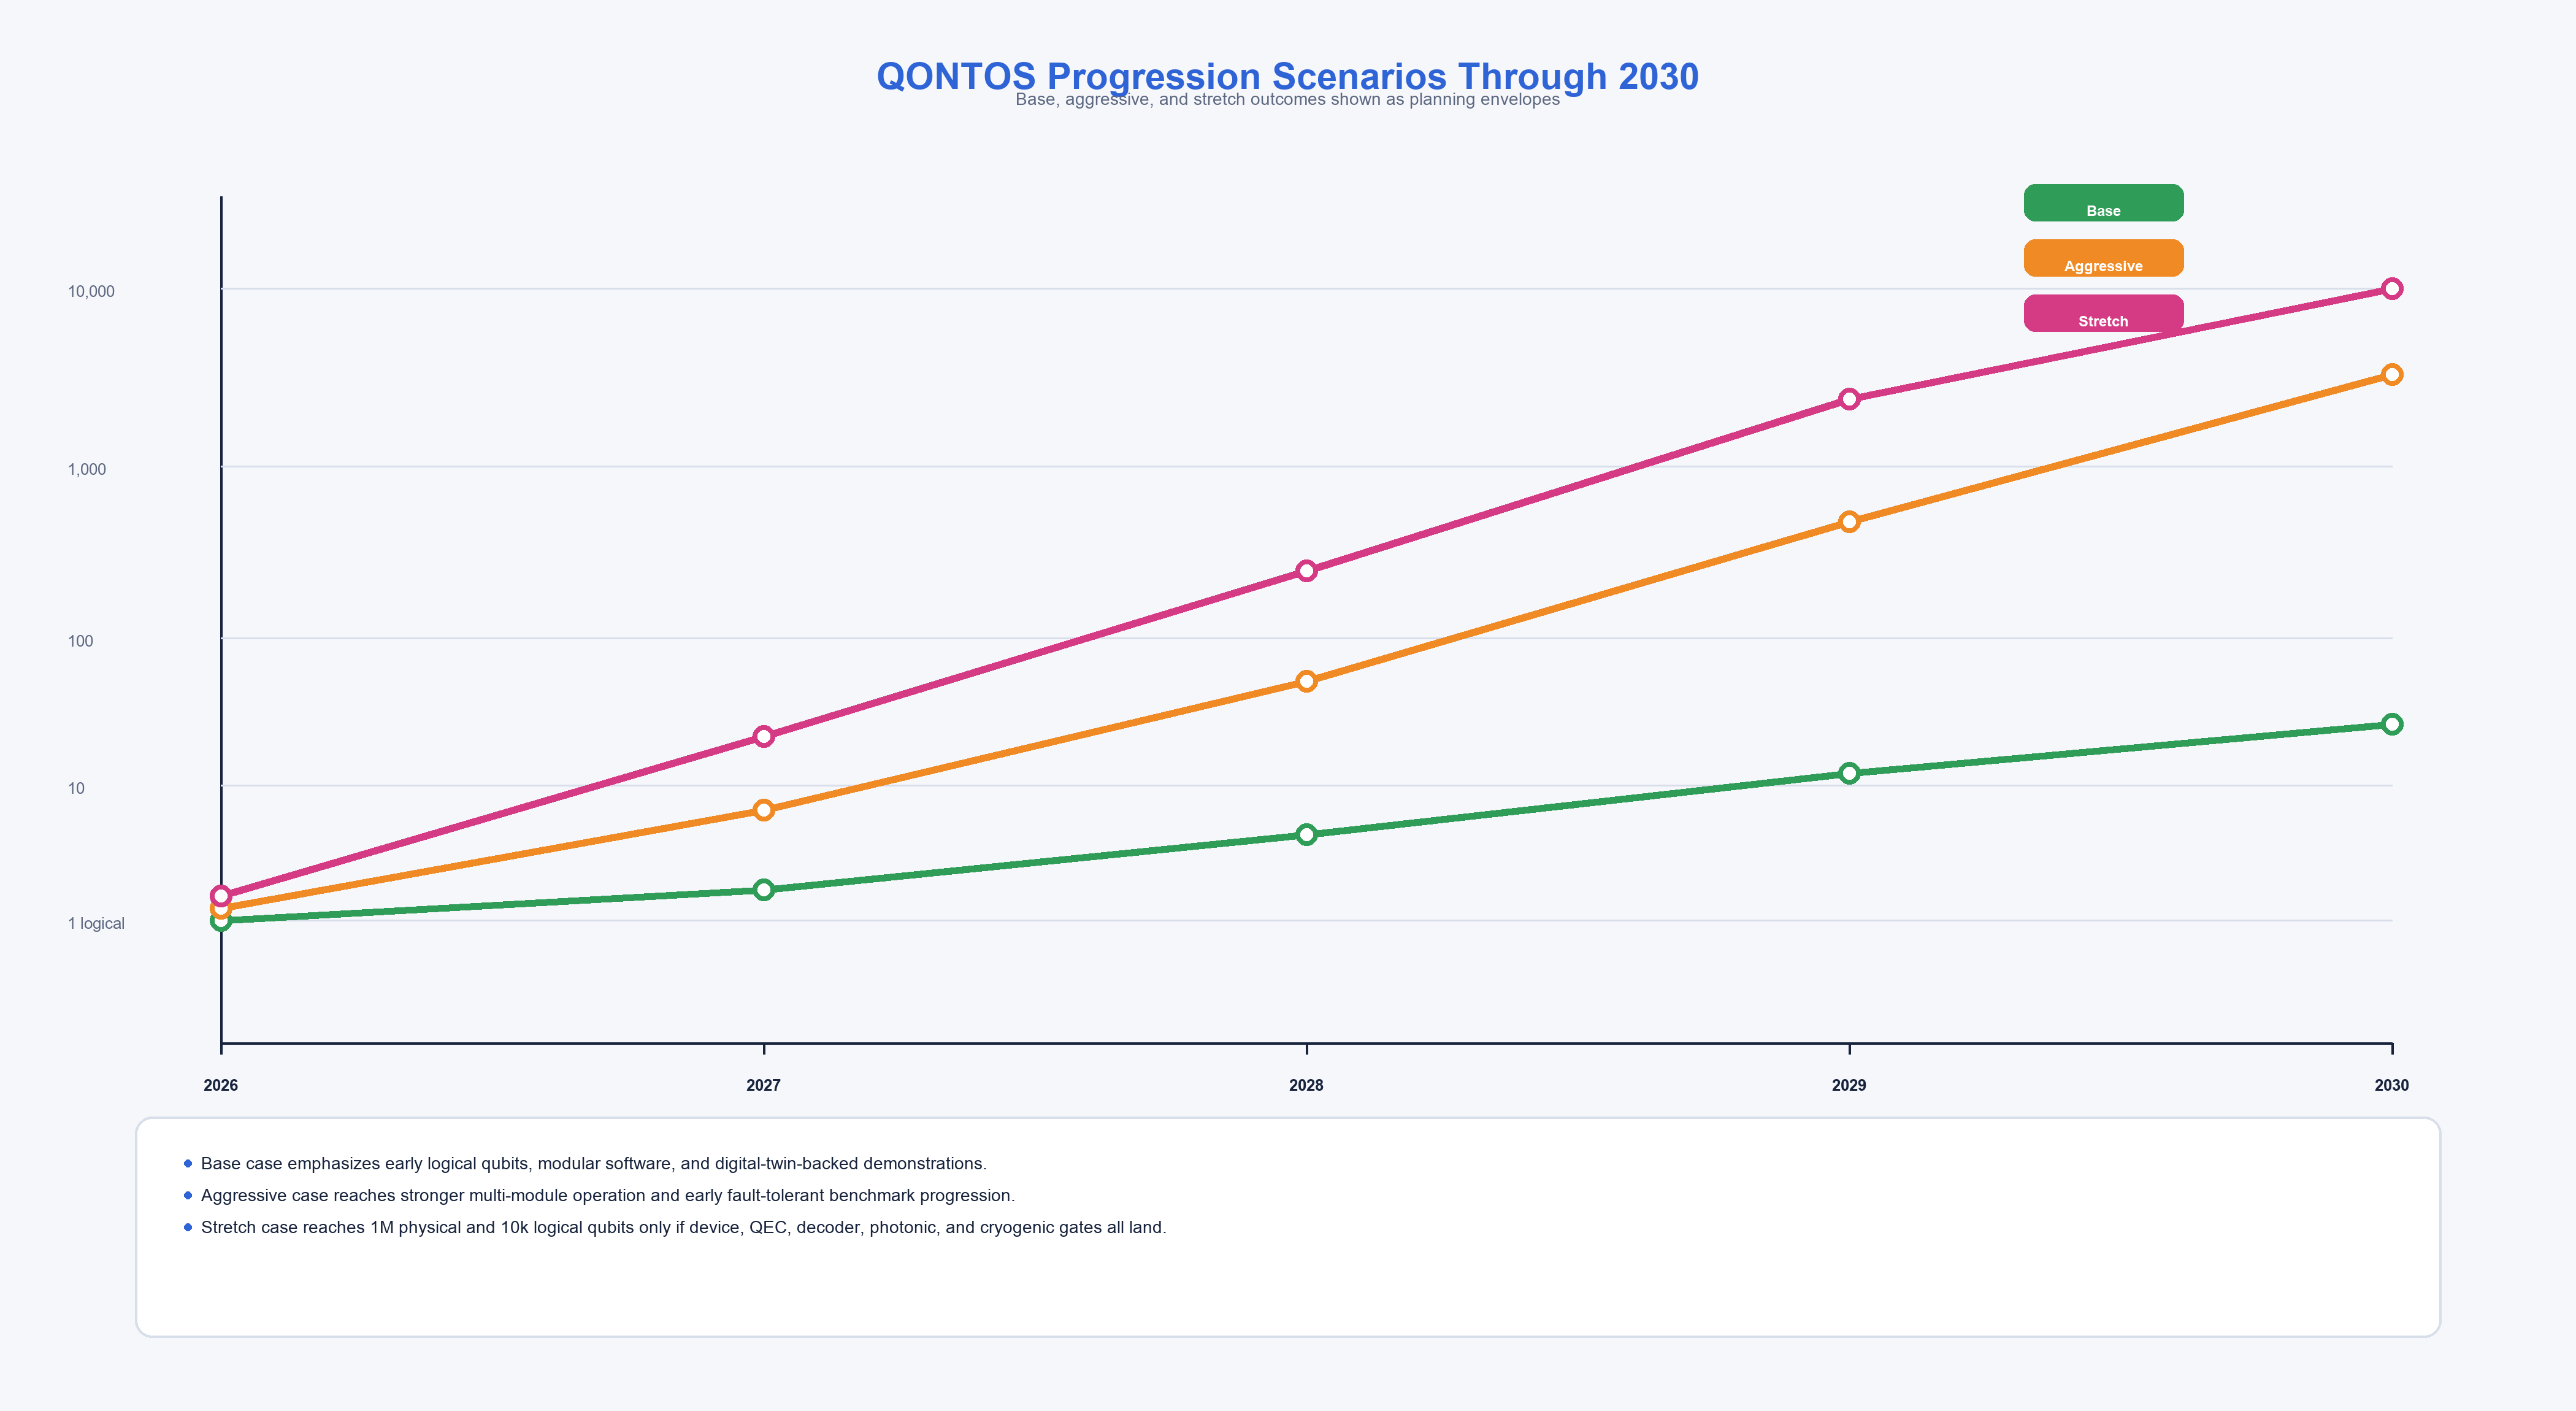
\includegraphics[width=\columnwidth]{../../figures/01_scaling_timeline.png}
\caption{Scaling Roadmap.}
\label{fig:roadmap}
\end{figure}

\subsection{Five Program Phases}

\begin{table*}[htbp]
\centering
\caption{Five Program Phases.}
\label{tab:phases}
\begin{tabular}{llp{3cm}p{3cm}p{3cm}}
\toprule
\textbf{Phase} & \textbf{Years} & \textbf{Base} & \textbf{Aggressive} & \textbf{Stretch} \\
\midrule
FOUNDATION & 2025--26 & Improved SW; digital twin; early device char. & First HW validation on QONTOS devices & Evidence toward ms-class coherence \\
SPUTNIK & 2026--27 & Small modular HW (2--5 chiplets); benchmarks & Scaled cryo module 5k+ qubits; first QEC & 10k phys.\ qubits/module; early logical \\
PIONEER & 2027--28 & Multi-module simulation; SW integration & Multi-module with photonic links; dist.\ runtime & 100k phys.\ qubits; 1k logical \\
HORIZON & 2028--29 & Robust modular control; partner-ready & Meaningful FTQC demos; app prototypes & 500k phys.\ qubits; 5k logical \\
SUMMIT & 2029--30 & Commercially useful sub-stretch; SW ecosystem & Large-scale logical platform; QA demos & 1M phys.\ qubits; 10k logical \\
\bottomrule
\end{tabular}
\end{table*}

\subsection{Phase-Gate Criteria}

\begin{table}[htbp]
\centering
\caption{Phase-Gate Criteria.}
\label{tab:phase_gates}
\begin{tabular}{lll}
\toprule
\textbf{Transition} & \textbf{Gate(s)} & \textbf{Decision} \\
\midrule
FOUND.$\to$SPUTNIK & G1 & Qubit quality OK? \\
SPUTNIK$\to$PIONEER & G2 & Logical qubit demo? \\
PIONEER$\to$HORIZON & G3 & Photonic links OK? \\
HORIZON$\to$SUMMIT & G4 + G5 & Models + economics OK? \\
\bottomrule
\end{tabular}
\end{table}

%% ----------------------------------------------------------------
\section{Competitive and Strategic Context}

\subsection{Monolithic vs.\ Modular Approaches}

\begin{table}[htbp]
\centering
\caption{Monolithic vs.\ Modular Comparison.}
\label{tab:mono_mod}
\begin{tabular}{lp{3.5cm}p{3.5cm}}
\toprule
\textbf{Approach} & \textbf{Advantages} & \textbf{Challenges} \\
\midrule
Monolithic & Simpler interconnect; lower latency; proven at current scale & Yield limits; thermal; wiring; freq.\ crowding \\
Modular & Relaxes per-chip limits; incremental upgrades; distributed arch. & Link fidelity; transduction; distributed control \\
\bottomrule
\end{tabular}
\end{table}

QONTOS's modular thesis is predicated on the argument that inter-module link challenges are more tractable in the long run than the combined monolithic scaling challenges at the 100,000+ qubit level. This argument is informed by published literature and engineering analysis, but it is not experimentally proven at the target scale.

\subsection{Industry Landscape}

The quantum computing field as of 2026 includes multiple hardware modalities and architectural philosophies:

\begin{itemize}
\item \textbf{Superconducting platforms} (Google, IBM, others) have demonstrated the most advanced error correction results to date~\cite{acharya2024, googleqai2023, krinner2022}.
\item \textbf{Trapped-ion platforms} offer high gate fidelities and all-to-all connectivity but face different scaling challenges related to trap complexity and ion transport.
\item \textbf{Neutral-atom platforms} have demonstrated rapid scaling of qubit count with reconfigurable connectivity.
\item \textbf{Photonic platforms} offer room-temperature operation but face challenges in deterministic entanglement generation.
\end{itemize}

The modular superconducting approach pursued by QONTOS is most directly comparable to IBM's quantum-centric supercomputing roadmap~\cite{ibm2024, ibm2024b}, though the specific architectural choices (chiplet size, module composition, interconnect technology) differ.

\subsection{Strategic Implications for QONTOS}

\begin{table}[htbp]
\centering
\caption{Strategic Position by Scenario.}
\label{tab:strategic}
\begin{tabular}{lp{5cm}}
\toprule
\textbf{Scenario} & \textbf{Strategic Position} \\
\midrule
Stretch & Full-stack modular QC with data-center-scale deployment \\
Aggressive & Leading modular platform with thousands of logical qubits \\
Base & Credible QC company with differentiated SW, digital twin, benchmarking \\
\bottomrule
\end{tabular}
\end{table}

The scenario framework ensures that QONTOS maintains a defensible strategic position across all three outcomes. The software-first foundation (orchestration, digital twin, benchmarking) retains value independent of the hardware scaling trajectory.

%% ----------------------------------------------------------------
\section{Conclusion}

This paper has defined the QONTOS modular quantum architecture as a structured engineering target with explicit assumptions, scenarios, validation criteria, dependencies, and risk factors. The principal conclusions are:

\begin{enumerate}
\item \textbf{The four-tier modular hierarchy} (chiplet / module / system / data center) provides a coherent composition framework with canonical constants of 2,000 / 10,000 / 100,000 / 1,000,000 physical qubits at the stretch level.

\item \textbf{The million-qubit, 10,000-logical-qubit endpoint is a stretch target} requiring simultaneous advances in qubit coherence~\cite{bland2025}, gate fidelity~\cite{acharya2024}, error-correction overhead~\cite{bravyi2024, fowler2012, panteleev2022}, photonic interconnects~\cite{monroe2014}, and classical decoding~\cite{krinner2022}. It should be understood as an aspirational planning target contingent on multiple linked subsystem breakthroughs.

\item \textbf{The three-scenario framework} (base / aggressive / stretch) provides resilience against technology shortfalls. Each scenario delivers a commercially meaningful outcome, and validation gates enable evidence-based trajectory adjustments.

\item \textbf{Identified dependencies and risks} (Sections~6--7) span qubit physics, integration engineering, cryogenics, and program execution. The modular architecture mitigates some risks (e.g., incremental scaling) while introducing others (e.g., inter-module link fidelity).

\item \textbf{The data center arithmetic is explicit and verified}: 10 systems of 100,000 qubits each yield 1,000,000 physical qubits. At 100:1 stretch overhead, this supports 10,000 logical qubits. At more conservative overhead ratios, fewer logical qubits are available, and the architecture delivers proportionally reduced computational capability.
\end{enumerate}

The value of this paper is not that it predicts or guarantees million-qubit delivery by 2030. Its value is that it defines a technically grounded target architecture, a canonical system ladder, a set of validation gates, and a comprehensive risk framework against which progress can be measured with intellectual honesty and engineering rigor.

%% ----------------------------------------------------------------
\appendices

\section{Notation and Abbreviations}

\begin{table}[htbp]
\centering
\caption{Abbreviations.}
\label{tab:abbrev}
\begin{tabular}{ll}
\toprule
\textbf{Abbrev.} & \textbf{Meaning} \\
\midrule
QEC & Quantum Error Correction \\
qLDPC & Quantum Low-Density Parity-Check (codes) \\
DR & Dilution Refrigerator \\
QPU & Quantum Processing Unit \\
FTQC & Fault-Tolerant Quantum Computing \\
$T_1$ & Energy relaxation time \\
$T_2$ & Dephasing time \\
2Q & Two-qubit (gate) \\
HPC & High-Performance Computing \\
MW & Microwave \\
ASIC & Application-Specific Integrated Circuit \\
FPGA & Field-Programmable Gate Array \\
EM & Electromagnetic \\
\bottomrule
\end{tabular}
\end{table}

\section{Claim Status Index}

Every major quantitative claim in this paper is indexed below with its status label.

\begin{table}[htbp]
\centering
\caption{Claim Status Index.}
\label{tab:claim_index}
\begin{tabular}{clp{2.5cm}}
\toprule
\textbf{Sec.} & \textbf{Claim} & \textbf{Status} \\
\midrule
3.1 & 2,000 qubits/chiplet & Stretch target \\
3.1 & 10,000 qubits/module & Stretch target \\
3.1 & 100,000 qubits/system & Stretch target \\
3.1 & 1,000,000 qubits/DC & Stretch target \\
3.1 & 10,000 logical @ 100:1 & Stretch target \\
3.2 & $T_1 > 2$~ms isolated & Demonstrated~\cite{bland2025} \\
3.2 & $T_1 > 1$~ms at scale & Stretch target \\
3.2 & 2Q fidelity $> 99.9\%$ & QONTOS target \\
3.2 & 2Q fidelity $> 99.99\%$ & Stretch target \\
4.1 & 1,000:1 overhead & Literature~\cite{fowler2012, chamberland2022} \\
4.1 & 300:1 overhead & QONTOS target \\
4.1 & 100:1 overhead & Stretch target \\
4.2 & qLDPC lower overhead & Literature~\cite{bravyi2024, panteleev2022} \\
5.1 & Base: 20k phys.\ qubits & QONTOS target \\
5.1 & Aggr.: 500k phys.\ qubits & QONTOS target \\
5.1 & Stretch: 1M phys.\ qubits & Stretch target \\
6.3 & ${\sim}1$~MW facility power & QONTOS target \\
6.3 & 100--200~m$^2$ footprint & QONTOS target \\
2.1 & Below-threshold SC op. & Demonstrated~\cite{acharya2024} \\
2.2 & Repeated QEC dist-3 & Demonstrated~\cite{krinner2022} \\
\bottomrule
\end{tabular}
\end{table}

%% ----------------------------------------------------------------
\bibliographystyle{IEEEtran}
\begin{thebibliography}{12}

\bibitem{bland2025}
S.~Bland \emph{et~al.}, ``Millisecond lifetimes and coherence times in 2D transmon qubits,'' \emph{Nature}, vol.~647, pp.~343--348, Nov. 2025.

\bibitem{acharya2024}
R.~Acharya \emph{et~al.} (Google Quantum AI), ``Quantum error correction below the surface code threshold,'' \emph{Nature}, vol.~634, pp.~834--840, 2024.

\bibitem{bravyi2024}
S.~Bravyi \emph{et~al.}, ``High-threshold and low-overhead fault-tolerant quantum memory,'' \emph{Nature}, vol.~627, pp.~778--782, 2024.

\bibitem{googleqai2023}
Google Quantum AI, ``Suppressing quantum errors by scaling a surface code logical qubit,'' \emph{Nature}, vol.~614, pp.~676--681, 2023.

\bibitem{monroe2014}
C.~Monroe, R.~Raussendorf, A.~Ruthven, K.~R. Brown, P.~Maunz, L.-M. Duan, and J.~Kim, ``Large-scale modular quantum-computer architecture with atomic memory and photonic interconnects,'' \emph{Phys.\ Rev.\ A}, vol.~89, p.~022317, 2014.

\bibitem{fowler2012}
A.~G. Fowler, M.~Mariantoni, J.~M. Martinis, and A.~N. Cleland, ``Surface codes: Towards practical large-scale quantum computation,'' \emph{Phys.\ Rev.\ A}, vol.~86, p.~032324, 2012.

\bibitem{koch2007}
J.~Koch \emph{et~al.}, ``Charge-insensitive qubit design derived from the Cooper pair box,'' \emph{Phys.\ Rev.\ A}, vol.~76, p.~042319, 2007.

\bibitem{ibm2024}
IBM, ``IBM Quantum Development and Innovation Roadmap,'' publicly available technical documentation, 2024.

\bibitem{krinner2022}
S.~Krinner \emph{et~al.}, ``Realizing repeated quantum error correction in a distance-three surface code,'' \emph{Nature}, vol.~605, pp.~669--674, 2022.

\bibitem{ibm2024b}
IBM Research, ``Quantum-centric supercomputing: The next wave of computing,'' IBM Research technical documentation, 2024.

\bibitem{chamberland2022}
C.~Chamberland \emph{et~al.}, ``Building a fault-tolerant quantum computer using concatenated cat codes,'' \emph{PRX Quantum}, vol.~3, p.~010329, 2022.

\bibitem{panteleev2022}
P.~Panteleev and G.~Kalachev, ``Asymptotically good quantum and locally testable classical LDPC codes,'' in \emph{Proc.\ 54th Annu.\ ACM Symp.\ Theory of Computing (STOC '22)}, pp.~375--388, 2022.

\end{thebibliography}

\end{document}
